\documentclass[DM,authoryear,toc]{lsstdoc}
% lsstdoc documentation: https://lsst-texmf.lsst.io/lsstdoc.html
\input{meta}

% Package imports go here.
\usepackage{listings}
\usepackage[section]{placeins}
\usepackage{authblk}
% Local commands go here.

%If you want glossaries
%\input{aglossary.tex}
%\makeglossaries

\title{Brighter-Fatter Correction GPU Optimization Using CUDA C/C++}

% Optional subtitle
% \setDocSubtitle{A subtitle}

%\author{Adriel Kim, Kevin Skadron, Eric Neilsen$^1$, and Michael Wang}
\author[1]{Adriel Kim}
\author[1]{Kevin Skadron}
\author[2]{Eric Neilsen}
\author[2]{Michael Wang}
\affil[1]{University of Virginia, Charlottesville, VA 22904, USA}
\affil[2]{Fermi National Accelerator Laboratory, Batavia, IL 60510, USA}

\setDocRef{RTN-015}
\setDocUpstreamLocation{\url{https://github.com/lsst/rtn-015}}

\date{\vcsDate}

% Optional: name of the document's curator
% \setDocCurator{The Curator of this Document}

\setDocAbstract{%
Leveraging the GPU with CUDA C/C++, the brighter-fatter effect (BFE) correction 
algorithm from the Large Synoptic Survey Telescope (LSST) Science Pipelines can 
be significantly optimized. BFE correction is among several other instrument
signature  removal (ISR) algorithms that are applied to astronomical images. BFE
correction  was a particularly good candidate for GPU optimization since it took
up a majority  of the ISR time (78.15\% of the total ISR time).
The BFE correction  algorithm itself is highly parallelizable, particularly due
to its use of convolutions  and NumPy functions such as numpy.diff and
numpy.gradient. Additionally, the algorithm  is an iterative process, which
offsets the time to perform memory transfers between  the CPU (host) and GPU
(device). The GPU implementation of the BFE correction algorithm  achieved an
average speed up of 10.95x over a CPU implementation using OpenCV C++.}

% Change history defined here.
% Order: oldest first.
% Fields: VERSION, DATE, DESCRIPTION, OWNER NAME.
% See LPM-51 for version number policy.
\setDocChangeRecord{%
  \addtohist{1}{2021-02-02}{Unreleased.}{Adriel Kim}
}

\begin{document}

% Create the title page.
\maketitle
% Frequently for a technote we do not want a title page  uncomment this to remove the title page and changelog.
% use \mkshorttitle to remove the extra pages

% ADD CONTENT HERE
% You can also use the \input command to include several content files.

\section{Introduction}

The LSST Science Pipelines are being developed in order to process astronomical data from LSST. The LSST is an exceptional telescope due to its wide field of view and its ability to survey the entire sky in just three nights. All this data must be processed before it can be searched for transients. This report is dealing specifically with the ISR tasks of this data. The ultimate purpose of this report is to provide a proof of concept of the speed up one can expect to achieve from optimizing a parallelizable algorithm in the LSST Science Pipelines. In addition, this report serves to provide a working GPU implementation of BFE correction that can be used as a guide for optimizing the LSST Science Pipelines in the future. Since the LSST Science Pipelines are being designed for the ``big data'' era, leveraging the GPU to speed up processing of large amounts of data would support this goal.

\section{Methods} 
\subsection{GPU Implementation}
In order to implement BFE correction with the GPU, the CUDA Toolkit 11.0 and NVIDIA 2D Image and Signal Performance Primitives (NPP) library were used. The CUDA Toolkit is the development environment used to write kernels, which are functions executed on the GPU. A 2D convolution filter from the NPP library was used to parallelize the convolution step of BFE correction. The following is a simple example of a CUDA kernel that adds two arrays in parallel.

\begin{lstlisting}[language=C++,basicstyle=\small,frame=single]
__global__ void matrixAddKernel(double *c, const double *a, const double *b) {
    int tid = threadIdx.x + blockIdx.x * blockDim.x;
    c[tid] = a[tid] + b[tid];
}
\end{lstlisting}

The following line of code launches the above kernel.

\begin{lstlisting}[language=C++,basicstyle=\small,frame=single]
matrixAddKernel << <blocksPerGrid, threadsPerBlock >> > (dev_c, dev_a, dev_b);
\end{lstlisting}

A kernel is launched with parameters (blocksPerGrid and threadsPerBlock) that determine how threads are grouped together. For each thread, the kernel above is executed. In this example, each thread is responsible for adding two individual elements. More information about kernels can be found in \cite{cudaex:2010}: \emph{CUDA by Example: An Introduction to General-Purpose GPU Programming}~.

The following is an actual sample of a CUDA kernel used to optimize BFE correction. This kernel implements the numpy.gradient function along the horizontal axis of a matrix.

\begin{lstlisting}[language=C++,basicstyle=\small,frame=single]
__global__ void matrixGradientKernel_2D_Row(float* c, const float* a) {
    int tid = threadIdx.x + blockIdx.x * blockDim.x; //current index
    
    int tid_row = tid / grad_C;
    int tid_col = tid % grad_C;
    
    if (tid_row == 0) {
        c[tid] = a[tid + grad_C] - a[tid];
    }
    else if (tid_col == grad_C-1) {
        c[tid] = a[tid] - a[tid - grad_C];
    }

    while (tid < grad_N - (2*grad_C)) {
        
        int tid_row_next = tid_row+2;
        int linear_index_next = (tid_row_next*grad_C)+tid_col;
        int linear_index_current = (tid_row * grad_C)+tid_col;

        c[tid + grad_C] = (a[linear_index_next] - a[linear_index_current])/2;        
        tid += blockDim.x * gridDim.x;
        tid_row = tid/grad_C;
        tid_col = tid%grad_C;
    }

}
\end{lstlisting}

A function such as numpy.gradient is easily parallelizable due to threads being independent from each other. In other words, communication between threads running in parallel is not needed to successfully get the gradient of a matrix. The following is what a CPU implementation of the above kernel could look like:

\begin{lstlisting}[language=C++,basicstyle=\small,frame=single]
void RowGradient(float* gradient_arr, float* spliced_arr, int startY,
                 int endY, int startX, int endX, int imgWidth) {

    float spliced_height = endY - startY;
    float spliced_width = endX - startX;
    float spliced_size = (spliced_height) * (spliced_width);

    for (int i = 0;i < spliced_width;i++) {
        int next_row = i + spliced_width;
        gradient_arr[i] = spliced_arr[next_row] - spliced_arr[i];
    }
    for (int i = spliced_size - spliced_width;i < spliced_size;i++) {
        int prev_row = i - spliced_width;
        gradient_arr[i] = spliced_arr[i] - spliced_arr[prev_row];
    }

    int row_offset = spliced_width;
  
    for (int row = 0;row < spliced_height - 2;row++) {
        for (int col = 0; col < spliced_width;col++) {
            int linear_index = (row * spliced_width) + col;
            int next_index = ((row + 2) * spliced_width) + col;

            gradient_arr[linear_index + row_offset] =
              (spliced_arr[next_index] - spliced_arr[linear_index]) / 2;
        }
    }
}
\end{lstlisting}

The following is another key CUDA kernel used in the optimized BFE correction. The kernel gets the sum of the absolute difference between two arrays.

\begin{lstlisting}[language=C++,basicstyle=\small,frame=single]
__global__ void matrixAbsDiffSum(float* c, const float* a, const float* b) {
    __shared__ float cache[threadsPerBlock];
    int tid = threadIdx.x + blockIdx.x * blockDim.x;
    int cacheIndex = threadIdx.x;

    float temp = 0;
    while (tid < N) {
        temp += abs(a[tid] - b[tid]);//absolute difference
        tid += blockDim.x * gridDim.x;
    }

    cache[cacheIndex] = temp;

    __syncthreads();

    int i = blockDim.x / 2;
    while (i != 0) {
        if (cacheIndex < i) {
            cache[cacheIndex] += cache[cacheIndex + i];
        }
        __syncthreads();
        i = i / 2;
    }
    if (cacheIndex == 0) {
        c[blockIdx.x] = cache[0];
    }
}
\end{lstlisting}

The previous example makes use of shared memory, which is memory shared among threads within the same thread block. This allows threads to cooperate with each other. In this particular example, each thread computes the absolute difference between corresponding elements from two different arrays. This value is then stored into the shared memory array called ``cache''. The kernel waits, using ``syncthreads()'', until all threads within the thread block have finished their computation. The last step is to perform a summation reduction using a technique outlined on page 79 of \cite{cudaex:2010}. The following is the CPU counterpart of the previous kernel:

\begin{lstlisting}[language=C++,basicstyle=\small,frame=single]
double MatrixAbsDiffSum(float* arr1, float* arr2, int arrSize) {
    double absDiff = 0;
    
    for (int i = 0;i < arrSize;i++) {
        absDiff += abs(arr1[i] - arr2[i]);
    }
    return absDiff;
}
\end{lstlisting}

\subsection{CPU Implementation}
The CPU implementation of BFE correction was created for the purposes of comparing the GPU counterpart against an already highly optimized library such as OpenCV, a computer vision and image processing library. The filter2D function from OpenCV was used to convolve the image, a key part of BFE correction. 

\section{Data}
\subsection{ISR Profiling Data}

\begin{table}[h]
\begin{center}
\begin{tabular}{|p{100pt}|p{150pt}|}
\multicolumn{2}{c}{\textbf{Times of Instrument Signature Removal Steps}}\\
\hline
ISR Step & Time (s)\\
\hline
1  float & 0 .06673 ( 0.4789\%)\\
\hline
2 overscan & 0.11245 ( 0.8069\%)\\
\hline
3 assemccd & 0.07163 ( 0.5140\%)\\
\hline
4 bias & 0.01806 ( 0.1296\%)\\
\hline
5 variance & 0.26160 ( 1.8772\%)\\
\hline
6 lin & 0.01767 ( 0.1268\%)\\
\hline
7 xtalk & 1.14747 ( 8.2339\%)\\
\hline
8 mskdef & 0.00111 ( 0.0080\%)\\
\hline
9 msknan & 0.01286 ( 0.0923\%)\\
\hline
10 widensat & 0.01511 ( 0.1084\%)\\
\hline
\textbf{11 bfcorr} & \textbf{10.89089 ( 78.1500\%)}\\
\hline
12 dark & 0.02414 ( 0.1732\%)\\
\hline
13 flat & 0.03530 ( 0.2533\%)\\
\hline
14 fringe & 0.00031 ( 0.0022\%)\\
\hline
15 vignette & 0.00072 ( 0.0052\%)\\
\hline
16 xcurves & 0.00006 ( 0.0004\%)\\
\hline
17 badreg & 0.20665 ( 1.4829\%)\\
\hline
18 interpmpix & 0.35914 ( 2.5771\%)\\
\hline
19 roughzp & 0.00006 ( 0.0004\%)\\
\hline
20 bkglevel & 0.69390 ( 4.9792\%)\\
\hline
Total & 13.93588\\
\hline
\end{tabular}
\caption{\label{tab:isrtimes}The table above contains all ISR steps along with their corresponding 
time and percentage of total time. This table helped identify the most time-consuming 
steps of the ISR process in order to narrow down candidates for GPU optimization. 
The data from the table was averaged over three different exposures. The BFE correction 
step (11 bfcorr), takes up 78.15\% of the total instrument signature removal process..}
\end{center}
\end{table}

\begin{figure}[h]
\centering
    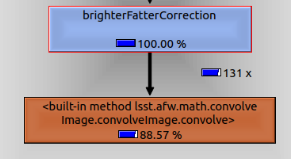
\includegraphics[width=0.4\textwidth]{./figs/profling.PNG}
\caption{The visualization above comes from a profiling of the ISR process using KCachegrind. This shows that the image convolution step within the BFE correction alone takes 88.57\% of the total time of the BFE correction step. This makes BFE correction a great candidate for GPU optimization since image convolution is already highly optimized on the GPU.}
\label{fig:kcachegrind}
\end{figure}

\clearpage

\subsection{Speed-up Results}

\begin{table}[h]
\begin{center}
\begin{tabular}{|p{47pt}|p{44pt}|p{45pt}|p{45pt}|p{45pt}|p{45pt}|}
\multicolumn{6}{c}{\textbf{GPU Timing Results}}\\
\multicolumn{2}{c}{\textbf{Exposure 1}} & \multicolumn{2}{c}{\textbf{Exposure 2}} &\multicolumn{2}{c}{\textbf{Exposure 3}}\\ 
\hline
Trial & Time (s) & Trial & Time (s) & Trial & Time (s)\\
\hline
1 & 0.693 & 1 & 0.739 & 1 & 0.711\\
\hline
2 & 0.704 & 2 & 0.679 & 2 & 0.754\\
\hline
3 & 0.696 & 3 & 0.663 & 3 & 0.682\\
\hline
4 & 0.685 & 4 & 0.708 & 4 & 0.691\\
\hline
5 & 0.692 & 5 & 0.697 & 5 & 0.695\\
\hline
6 & 0.706 & 6 & 0.698 & 6 & 0.689\\
\hline
7 & 0.694 & 7 & 0.694 & 7 & 0.715\\
\hline
8 & 0.69 & 8 & 0.698 & 8 & 0.696\\
\hline
9 & 0.682 & 9 & 0.702 & 9 & 0.704\\
\hline
10 & 0.692 & 10 & 0.704 & 10 & 0.715\\
\hline
\textbf{Average:} & \textbf{0.6934} & \textbf{Average:} & \textbf{0.6982} & \textbf{Average:} & \textbf{0.7052}\\
\hline
\textbf{Speed up over OpenCV:} & \textbf{11.027} & \textbf{Speed up over OpenCV:} & \textbf{10.968} & \textbf{Speed up over OpenCV:} & \textbf{10.854}\\
\hline
\multicolumn{3}{l}{\textbf{Average Speed up: 10.95}}&\multicolumn{3}{c}{}\\
\end{tabular}
\caption{\label{tab:gputimes}GPU implementation of brighter-fatter timing and speed-up}
\end{center}
\end{table}

\begin{table}[h]
\begin{center}
\begin{tabular}{|p{45pt}|p{45pt}|p{45pt}|p{45pt}|p{45pt}|p{45pt}|}
\multicolumn{6}{c}{\textbf{CPU Timing Results}}\\
\multicolumn{2}{c}{\textbf{Exposure 1}} & \multicolumn{2}{c}{\textbf{Exposure 2}} &\multicolumn{2}{c}{\textbf{Exposure 3}}\\ 
\hline
Trial & Time (s) & Trial & Time (s) & Trial & Time (s)\\
\hline
1 & 7.644 & 1 & 7.643 & 1 & 7.668\\
\hline
2 & 7.668 & 2 & 7.608 & 2 & 7.681\\
\hline
3 & 7.647 & 3 & 7.656 & 3 & 7.669\\
\hline
4 & 7.609 & 4 & 7.681 & 4 & 7.677\\
\hline
5 & 7.628 & 5 & 7.677 & 5 & 7.658\\
\hline
6 & 7.649 & 6 & 7.669 & 6 & 7.652\\
\hline
7 & 7.639 & 7 & 7.678 & 7 & 7.644\\
\hline
8 & 7.641 & 8 & 7.662 & 8 & 7.638\\
\hline
9 & 7.668 & 9 & 7.64 & 9 & 7.64\\
\hline
10 & 7.673 & 10 & 7.669 & 10 & 7.621\\
\hline
\textbf{Average:} & \textbf{7.6466} & \textbf{Average:} & \textbf{7.6583} & \textbf{Average:} & \textbf{7.6548}\\
\hline
\end{tabular}
\caption{\label{tab:cputimes}CPU implementation of brighter-fatter timing.}
\end{center}
\end{table}

\FloatBarrier

\clearpage
\subsection{Image Comparisons}

\begin{figure}[h]
\centering
  \begin{tabular}[t]{cc}
    \textbf{Input Image Before BFE Correction} & \textbf{Output Image After BFE Correction}\\
    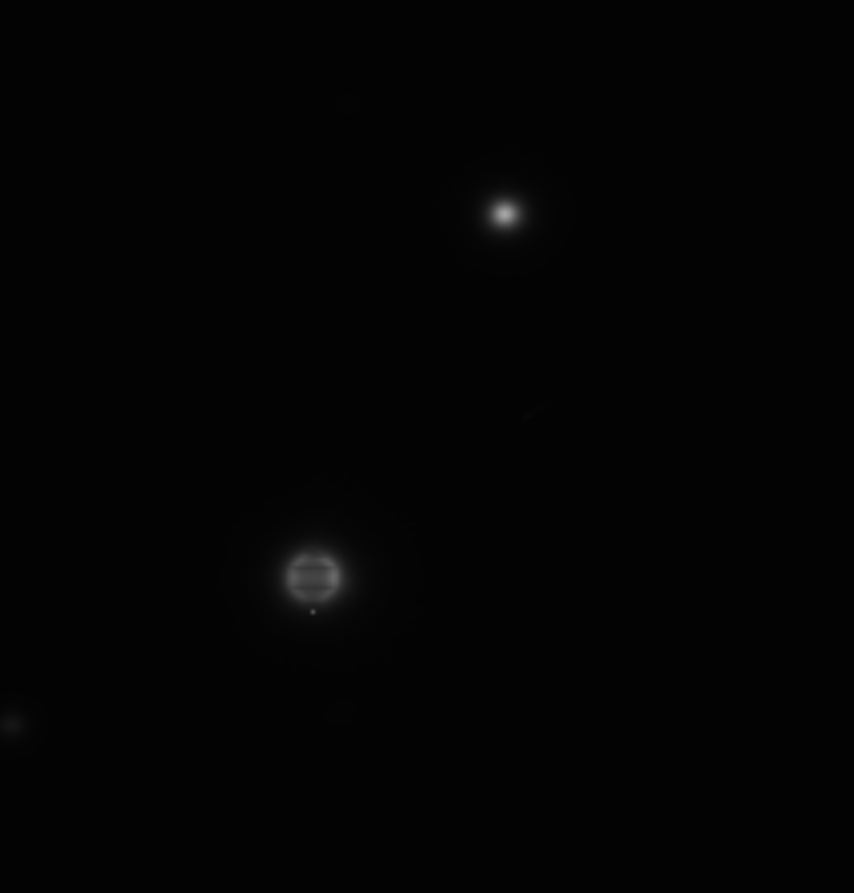
\includegraphics[trim=5.55cm 5.35cm 7.1cm 3.25cm,clip=true,width=0.45\textwidth]{./figs/fig15/input_snippet.png} &
    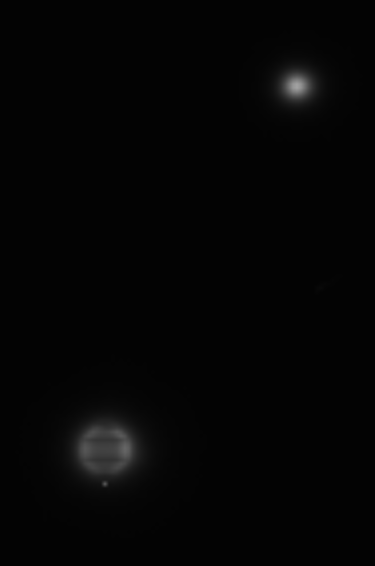
\includegraphics[width=0.45\textwidth]{./figs/fig15/LSST_ouput_snippet.png} \\
  \end{tabular}
\caption{The table above shows the original input image and the corresponding output image after BFE correction. For demonstration purposes, only a small snippet of the actual images are seen there. This table is not very useful since it's difficult to tell the difference by eye alone. However, the input and output images can be subtracted to observe the differences between them.}
\label{fig:bfeinvsout}
\end{figure}

\begin{figure}[h]
\centering
  \begin{tabular}[t]{ccc}
    \textbf{LSST Science Pipelines} & \textbf{GPU Optimized} & \textbf{Difference between}\\
    \textbf{Difference Between Before} & \textbf{Difference Between Before}& \textbf{GPU and CPU (LSST}\\
    \textbf{and After BFE Correction}  & \textbf{and After BFE Correction} & \textbf{Science Pipelines) Result}\\
    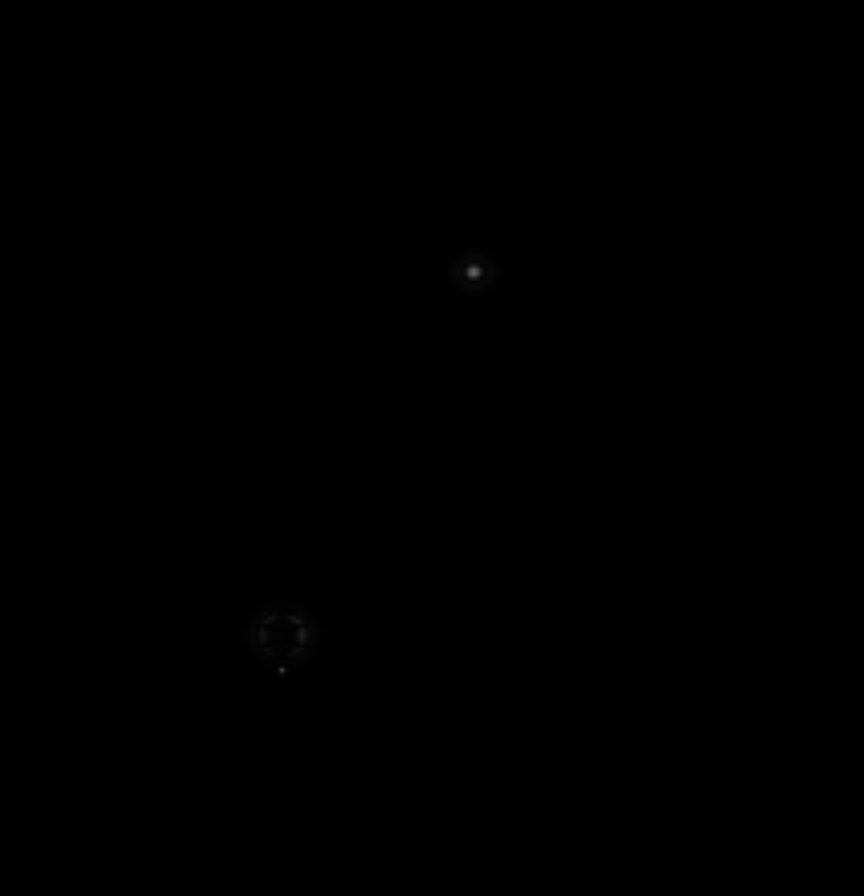
\includegraphics[trim=4cm 3.7cm 8cm 4.5cm,clip=true,width=0.3\textwidth]{./figs/fig16/LSST_input_output_difference_snippet.png} &
    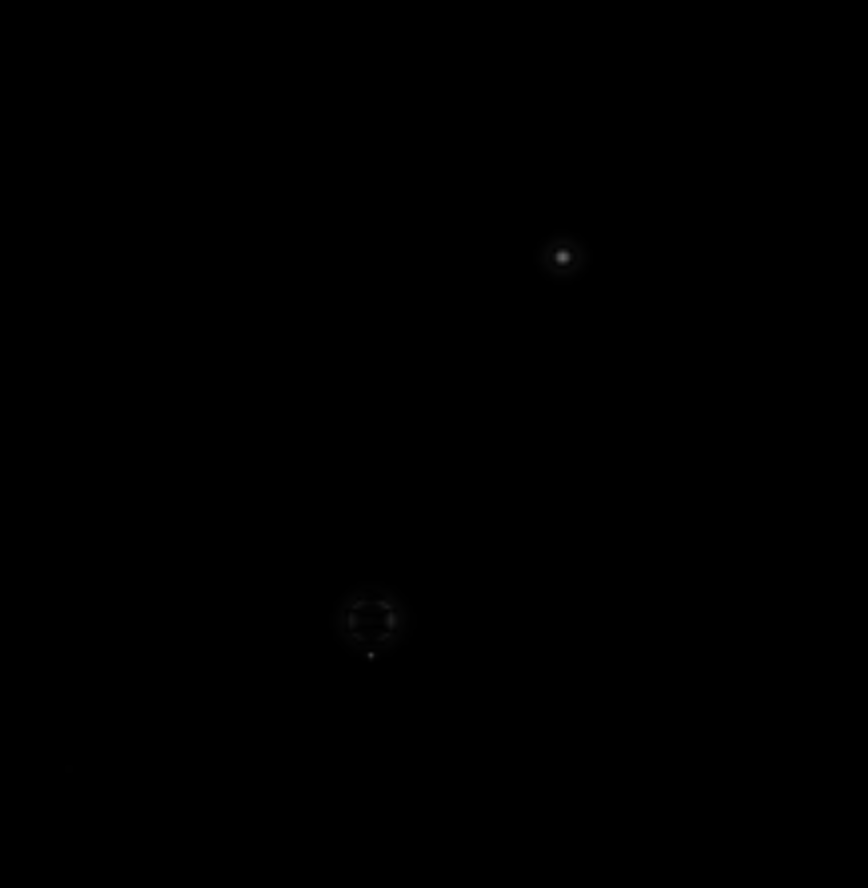
\includegraphics[trim=6.5cm 3.8cm 5.5cm 4.1cm,clip=true,width=0.3\textwidth]{./figs/fig16/GPU_input_output_difference_snippet.png} &
    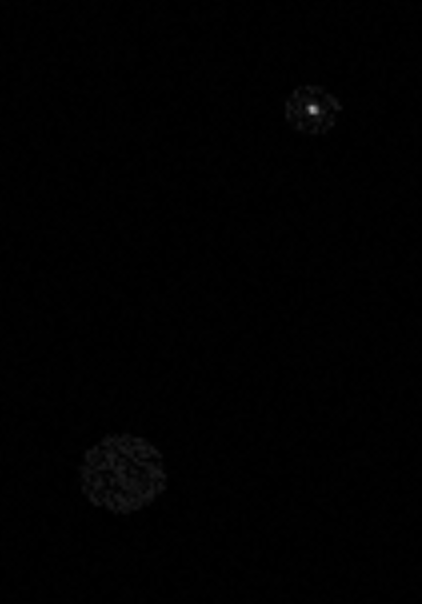
\includegraphics[width=0.3\textwidth]{./figs/fig16/LSST_GPU_error_snippet.png} \\
  \end{tabular}
\caption{The table above shows the difference between the input and output images of both the original BFE correction from the LSST Science Pipelines and the GPU optimized version. Visually, this demonstrates that the original BFE correction and the GPU optimized version produce similar results. The last column in the table shows the difference between the GPU result and LSST's CPU result. Visually, this shows the error of the GPU result. Note, the images above were brightened so that they could be seen more easily.}
\label{fig:bfediff}
\end{figure}

\begin{figure}[h]
\centering
  \begin{tabular}[t]{c}
    \textbf{GPU Result Max Absolute Error}\\
    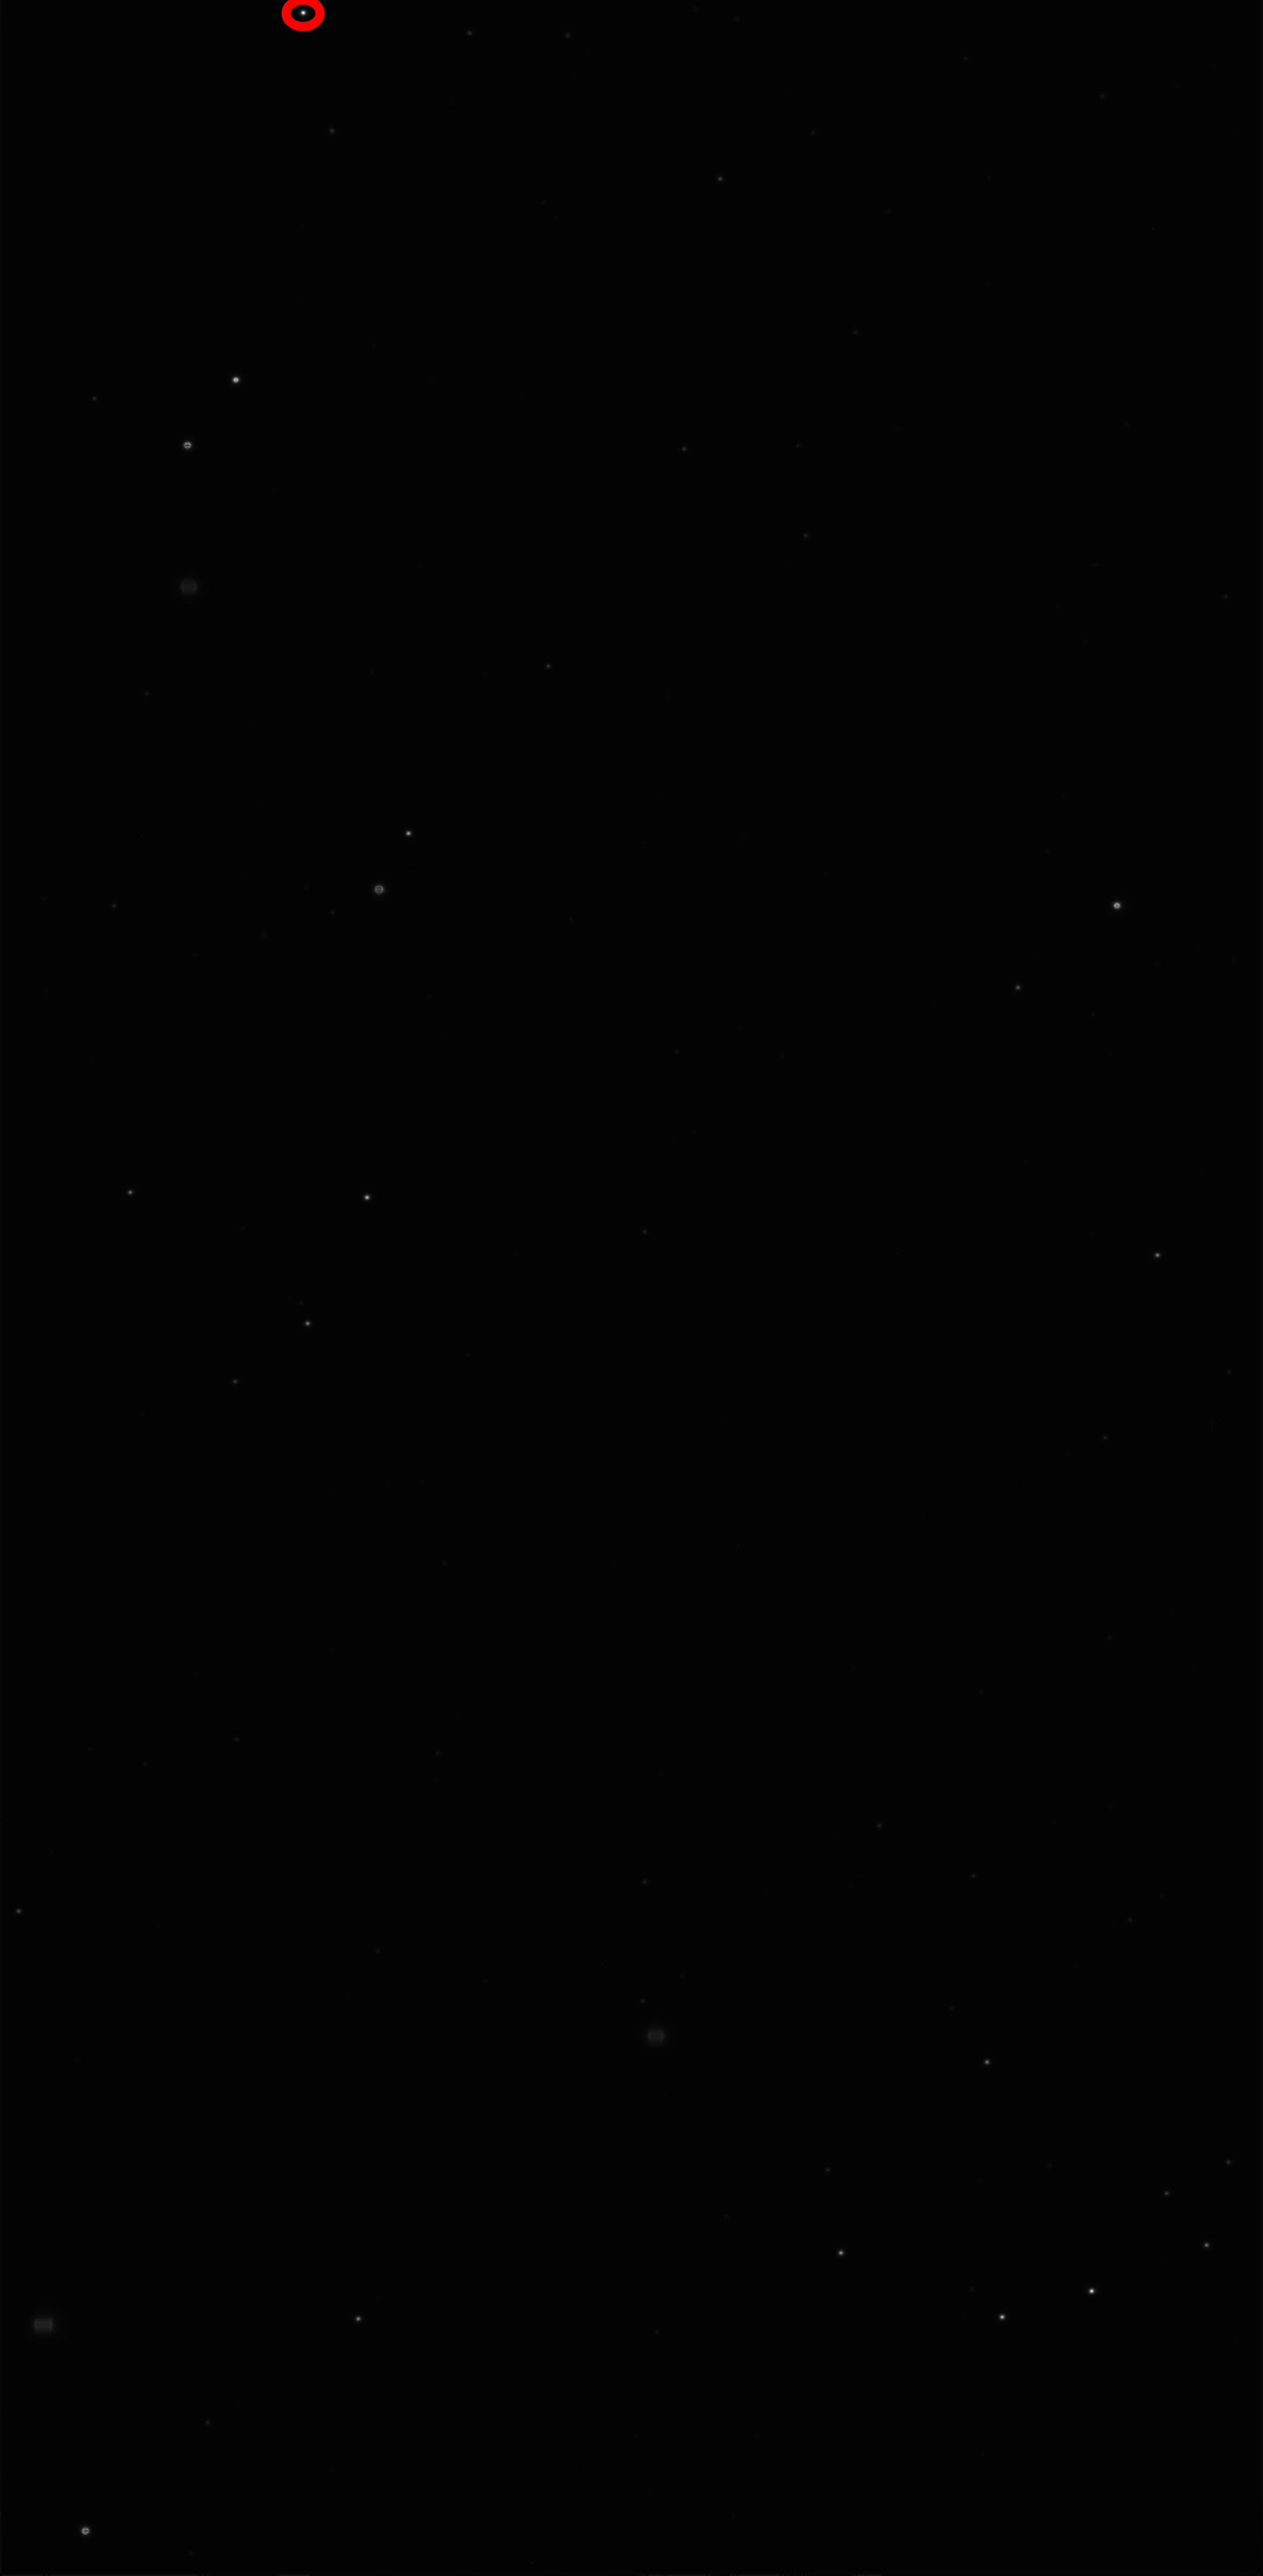
\includegraphics[trim=0cm 95cm 0cm 0cm,clip=true,width=0.9\textwidth]{./figs/fig17/max_error_GPU_labeled.png}\\
  \end{tabular}
\caption{This is the cropped upper part of the resulting GPU image of exposure 1. Circled in red is the location of max absolute error,
where a star is located (See Table~\ref{tab:gpuerrcorrimg} for max absolute error)}
\label{fig:bfemaxerr}
\end{figure}

\FloatBarrier

\clearpage

\subsection{Image Error}

\begin{table}[h]
\begin{center}
\begin{tabular}{|c|c|c|c|}
\multicolumn{4}{c}{\textbf{GPU Implementation Error of BFE Corrected Image}}\\
\hline
 & Mean Squared & Max Error Percent & Max Absolute\\
 & Error (MSE) & & Error\\
\hline
Exposure 1 & 3.27E-08 & 7.28E-07 & 0.09375\\
\hline
Exposure 2 & 3.98E-08 & 7.15E-07 & 0.125\\
\hline
Exposure 3 & 1.52E-08 & 6.01E-07 & 0.0703125\\
\hline
\textbf{Average} & \textbf{2.93E-08} & \textbf{6.81E-07} & \textbf{0.096}\\
\hline
\end{tabular}
\caption{\label{tab:gpuerrcorrimg}Error of resulting image from GPU implementation for three different input exposures.}
\end{center}
\end{table}


\begin{table}[h]
\begin{center}
\begin{tabular}{|c|c|c|}
\multicolumn{3}{c}{\textbf{GPU Implementation Error of Correction Matrix}}\\
\hline
 & Correction Matrix MSE & Correction Matrix Max Absolute Error\\
\hline
Exposure 1 & 2.82E-08 & 0.102051\\
\hline
Exposure 2 & 3.52E-08 & 0.115723\\
\hline
Exposure 3 & 1.10E-08 & 0.0651855\\
\hline
\textbf{Average} & \textbf{2.48E-08} & \textbf{0.094}\\
\hline
\end{tabular}
\caption{\label{tab:gpuerrcorrmat}Error of resulting correction matrix from GPU implementation for three different input exposures. The correction matrix is the matrix added to the original image to correct for the BFE.}
\end{center}
\end{table}

\begin{table}[h]
\begin{center}
\begin{tabular}{|c|c|c|c|}
\multicolumn{4}{c}{\textbf{CPU Implementation Error of BFE Corrected Image}}\\
\hline
 & Mean Squared & Max Error Percent & Max Absolute\\
 & Error (MSE) & & Error\\
\hline
Exposure 1 & 3.65E-09 & 1.85E-07 & 0.015625\\
\hline
Exposure 2 & 4.21E-09 & 2.29E-07 & 0.0234375\\
\hline
Exposure 3 & 2.63E-09 & 2.16E-07 & 0.03125\\
\hline
\textbf{Average} & \textbf{3.49E-09} & \textbf{2.10E-07} & \textbf{0.023}\\
\hline
\end{tabular}
\caption{\label{tab:cpuerrcorrimg}Error of resulting image from GPU implementation for three different input exposures.
}
\end{center}
\end{table}

\begin{table}[h]
\begin{center}
\begin{tabular}{|c|c|c|}
\multicolumn{3}{c}{\textbf{CPU Implementation Error of Correction Matrix}}\\
\hline
 & Correction Matrix MSE & Correction Matrix Max Absolute Error\\
\hline
Exposure 1 & 1.85E-09 & 0.027832\\
\hline
Exposure 2 & 2.33E-09 & 0.0273438\\
\hline
Exposure 3 & 1.07E-09 & 0.0283203\\
\hline
\textbf{Average} & \textbf{1.75E-09} & \textbf{0.028}\\
\hline
\end{tabular}
\caption{\label{tab:cpuerrcorrmat}Error of resulting correction matrix from CPU implementation for three different input exposures.}
\end{center}
\end{table}


\section{Disclaimer}
The code written for the purposes of this report are standalone versions of the BFE correction algorithm to demonstrate whether or not speed up with the GPU is potentially effective. It has not been designed to be integrated in the LSST Science Pipelines, nor has it been tested along with all the ISR steps. In addition, the CPU code may not be highly optimized with the exception of the filter2D function from OpenCV. There may be other CPU implementations of BFE correction that would run in less time and result in less speed up from the GPU. Likewise, the GPU code may not be highly optimized with the exception of NPP's filter function. Thus, the actual speed up results may either be higher or lower than what was shown in this report.

\section{Conclusion}

The LSST Science Pipelines will need to be able to handle large amounts of data efficiently. Using a parallel computing platform, such as CUDA C/C++, is a viable way to optimize the codebase as demonstrated by the nearly 11x speed up achieved by a GPU implementation of the BFE correction algorithm. 

\section{Code and Figures}

The figures and code for both the GPU and CPU implementations of BFE correction can be found in this Github repository:\newline
\url{https://github.com/adrielk/LSST-Brighter-Fatter-GPU-Optimization}

\appendix
% Include all the relevant bib files.
% https://lsst-texmf.lsst.io/lsstdoc.html#bibliographies
\section{References} \label{sec:bib}
\renewcommand{\refname}{} % Suppress default Bibliography section
\bibliography{local,lsst,lsst-dm,refs_ads,refs,books}

% Make sure lsst-texmf/bin/generateAcronyms.py is in your path
\section{Acronyms} \label{sec:acronyms}
\addtocounter{table}{-1}
\begin{longtable}{p{0.145\textwidth}p{0.8\textwidth}}\hline
\textbf{Acronym} & \textbf{Description}  \\\hline

2D & Two-dimensional \\\hline
CPU & Central Processing Unit \\\hline
DM & Data Management \\\hline
GPU & Graphics Processing Unit \\\hline
ISR & Instrument Signal Removal \\\hline
LSST & Legacy Survey of Space and Time (formerly Large Synoptic Survey Telescope) \\\hline
RTN & Rubin Technical Note \\\hline
\end{longtable}

% If you want glossary uncomment below -- comment out the two lines above
%\printglossaries

\section{Acknowledgements} \label{sec:acknowledgement}

This manuscript has been authored by Fermi Research Alliance, LLC under Contract No. DE-AC02-07CH11359 with the U.S. Department of Energy, Office of Science, Office of High Energy Physics.


\end{document}
